\chapter{Выполнение лабораторной работы}

\section{Цель работы}

Лабораторная работа № 3 нацелена на отработку навыков использования программы
Microsoft Project для оптимизации временных и финансовых показателей
проекта.

\section{Краткое описание проекта}

Команда разработчиков из 16 человек занимается созданием карты города на основе собственного модуля отображения. Проект должен быть завершен в течение 6 месяцев. Бюджет проекта: 50 000 рублей.

\section{Задание 1}

Ликвидировать перегрузку ресурсов в проекте. Для ликвидации перегрузки использовалось автоматическое выравнивание. Результаты выравнивания представлены на рисунке~\ref{fig:sved}

\begin{figure}[H]
	\centering
	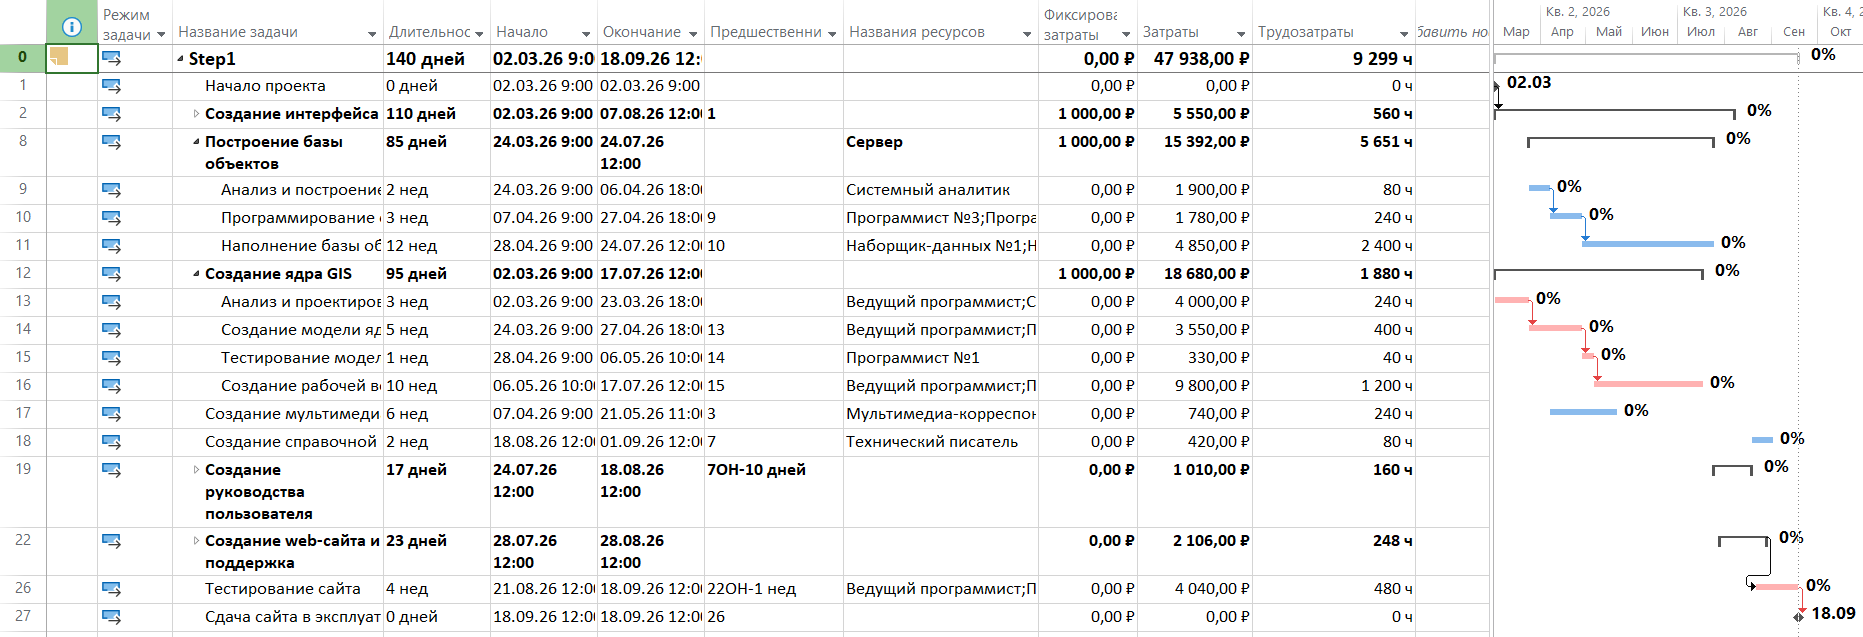
\includegraphics[width=\linewidth]{images/after_vir_1.png}
	\caption{План работ и диаграмма Ганта после применения автоматического выравнивания}
	\label{fig:sved}
\end{figure}

Срок окончания работ сдвинулся на два дня, в связи с тем, что обе выполняемые художником-дизайнером параллельно задачи находились на критическом пути. Кроме того, сервер работает на день меньше в связи с изменением дат начала и окончания выполнения работ по построению базы объектов, что привело к сокращению затрат на 48 рублей.

\section{Задание 2}

Отразить в плане проекта проведение еженедельного совещания по средам с 10 до 11 утра. Результат добавления совещания представлен на рисунках~\ref{fig:2} и~\ref{fig:3}. 

\begin{figure}[H]
	\centering
	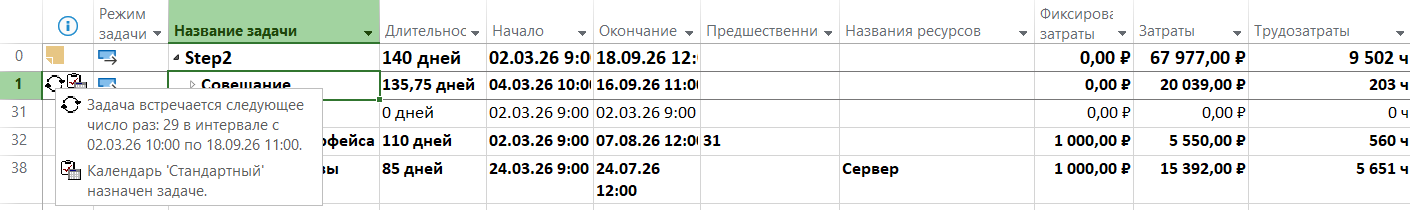
\includegraphics[width=\linewidth]{images/hueta.png}
	\caption{Общая задача проекта и повторяющаяся задача "Совещание"}
	\label{fig:2}
\end{figure}

\begin{figure}[H]
	\centering
	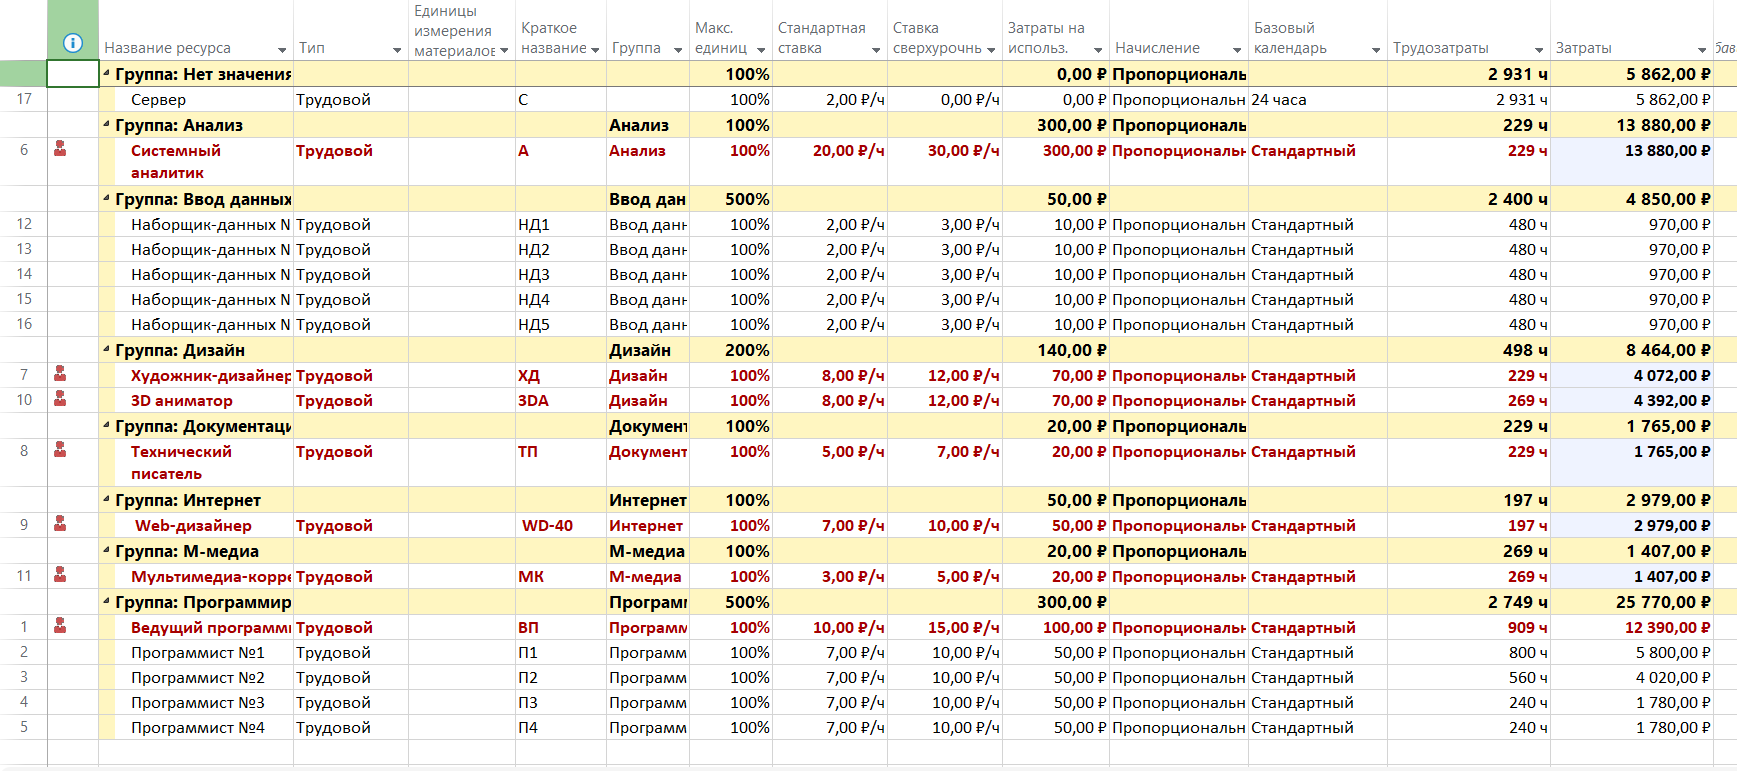
\includegraphics[width=\linewidth]{images/hueta_1.png}
	\caption{Сгруппированные ресурсы после добавления повторяющейся задачи}
	\label{fig:3}
\end{figure}

В результате добавление совещания трудозатраты увелчились на 203 часа, а затраты на 20039 рублей. Также возникла перегрузка сотрудников участвующих в совещании, в связи дополнительным рабочим часом в день.

После устранения перегрузки с использование автоматического выравнивания, дата окончания проекта сдвинулась на 23.09, трудозатраты выросли на 3 часа, затраты~---~на 6 рублей, в связи с тремя дополнительными часами работы сервера. Соответствующие результаты отображены на рисунках~\ref{fig:4} и~\ref{fig:5}.

\begin{figure}[H]
	\centering
	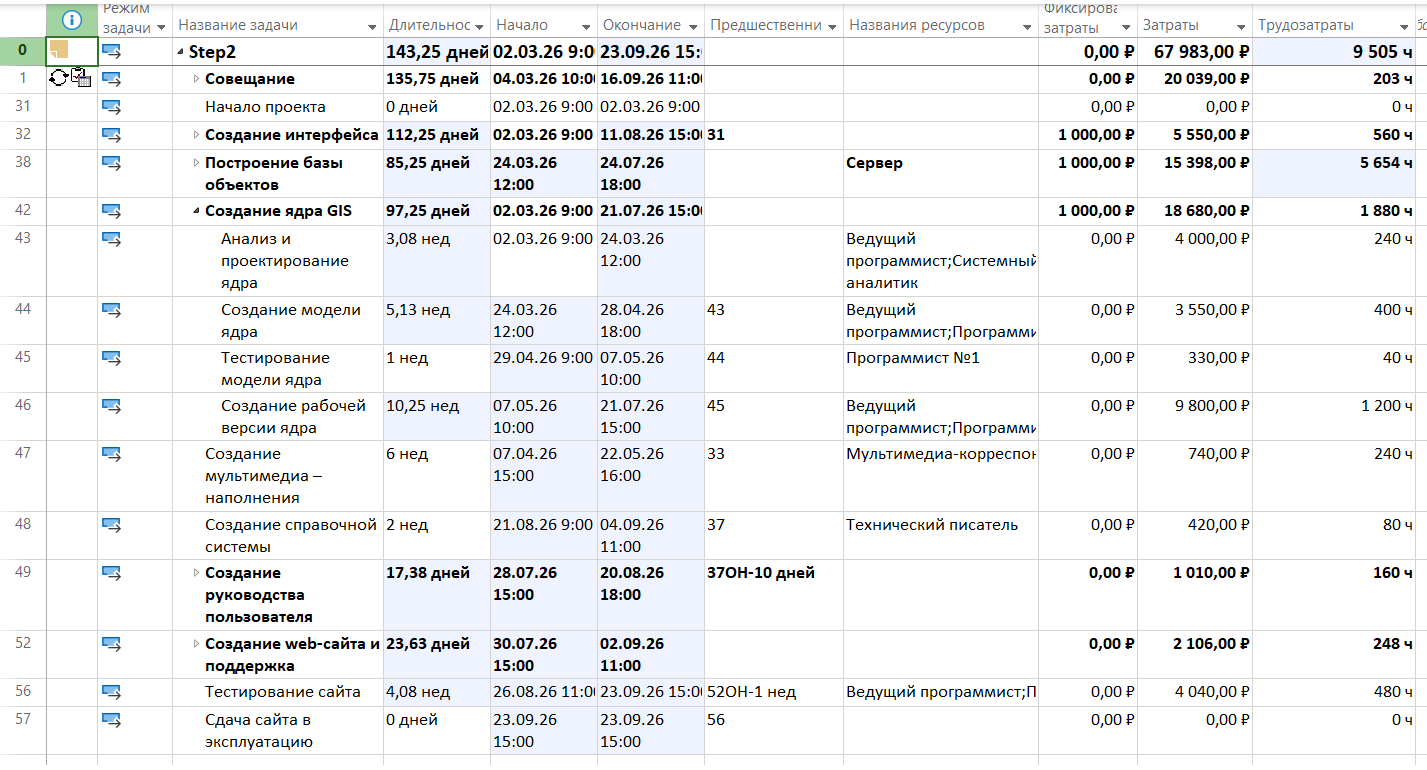
\includegraphics[width=\linewidth]{images/sov_i_vir.png}
	\caption{План работ после применения автоматического выравнивания}
	\label{fig:4}
\end{figure}

\begin{figure}[H]
	\centering
	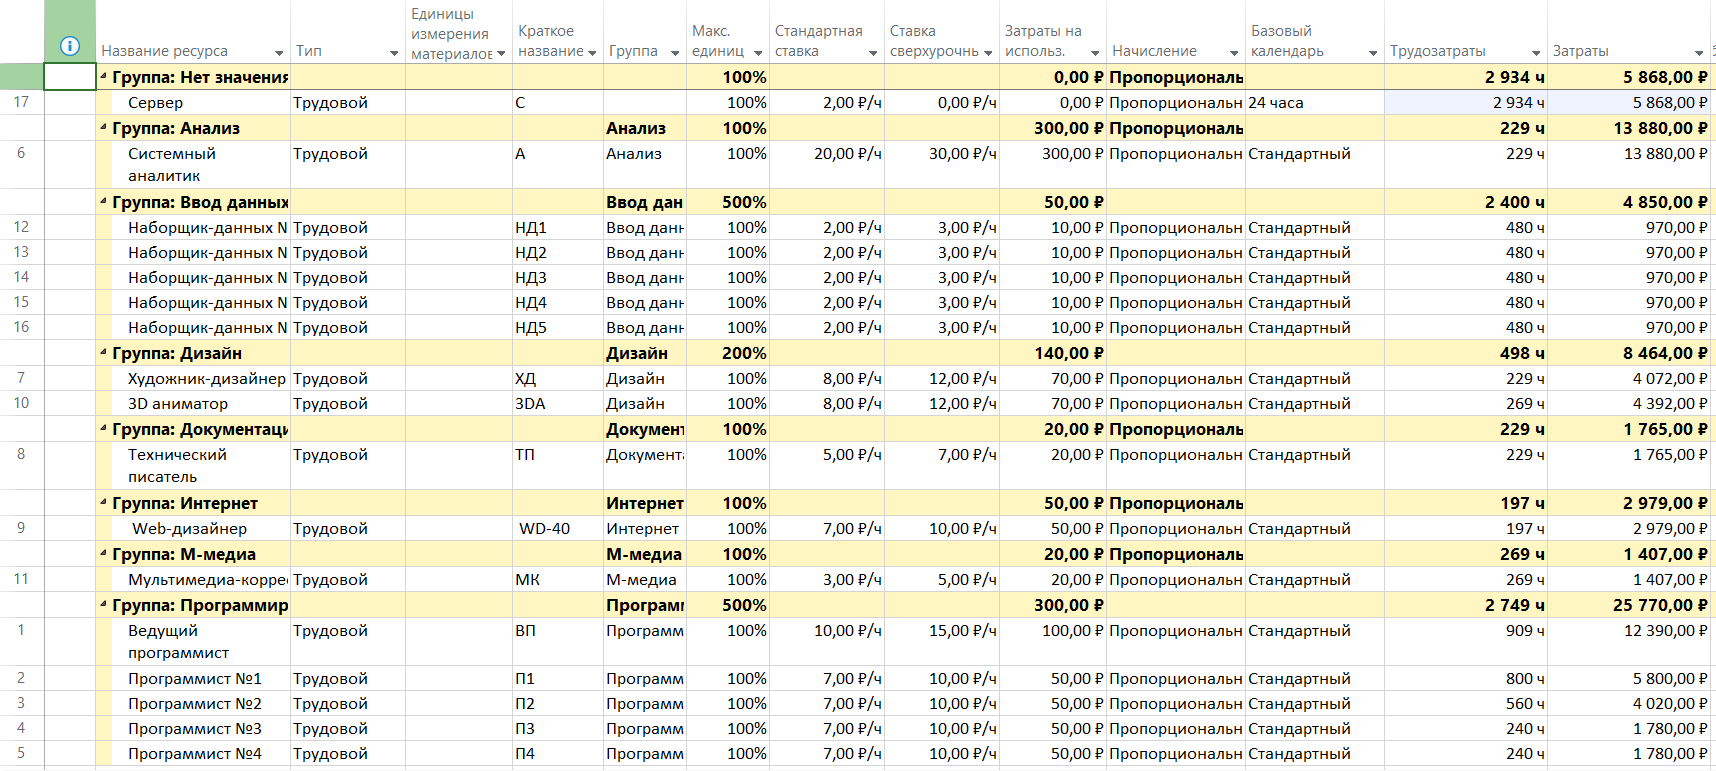
\includegraphics[width=\linewidth]{images/sov_i_vir_1.png}
	\caption{Сгруппированные ресурсы после применения автоматического выравнивания}
	\label{fig:5}
\end{figure}

В связи с превышением бюджета на 17983 рубля и сроков завершения проекта на 21 день, необходимо провести оптимизацию временных и финансовых затрат проекта. Для этого на задачи <<Программирование средств обработки базы объектов>>, <<Тестирование сайта>>, <<Программирование интерфейса>>, <<Тестирование модели ядра>> и <<Создание модели ядра>> были назначены все имеющиеся программисты. Дополнительно с задачи <<Тестирование сайта>> был снят ведущий программист. После этого устранены появившиеся перегрузки с помощью автоматического выравнивания, а также убраны совещания, после окончания работ по задачам.

Дополнительно к этому, для сотрудников участвующих в совещании настроена дополнительная таблица норм затрат, в которой исключены затраты на использование сотрудника, в связи с тем, что во время совещания сотрудник не использует свое рабочее место.

Результаты принятых мер оптимизации представлены на рисунках~\ref{fig:6} и~\ref{fig:7}.

\begin{figure}[H]
	\centering
	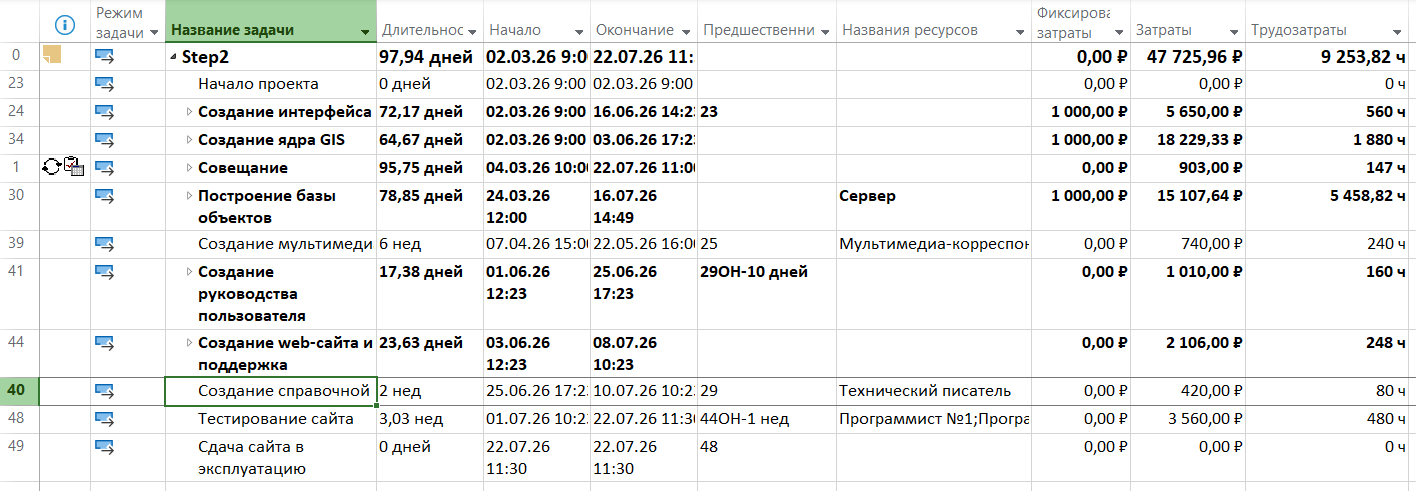
\includegraphics[width=\linewidth]{images/final_ochka.png}
	\caption{План работ после применения мер оптимизации}
	\label{fig:6}
\end{figure}

\begin{figure}[H]
	\centering
	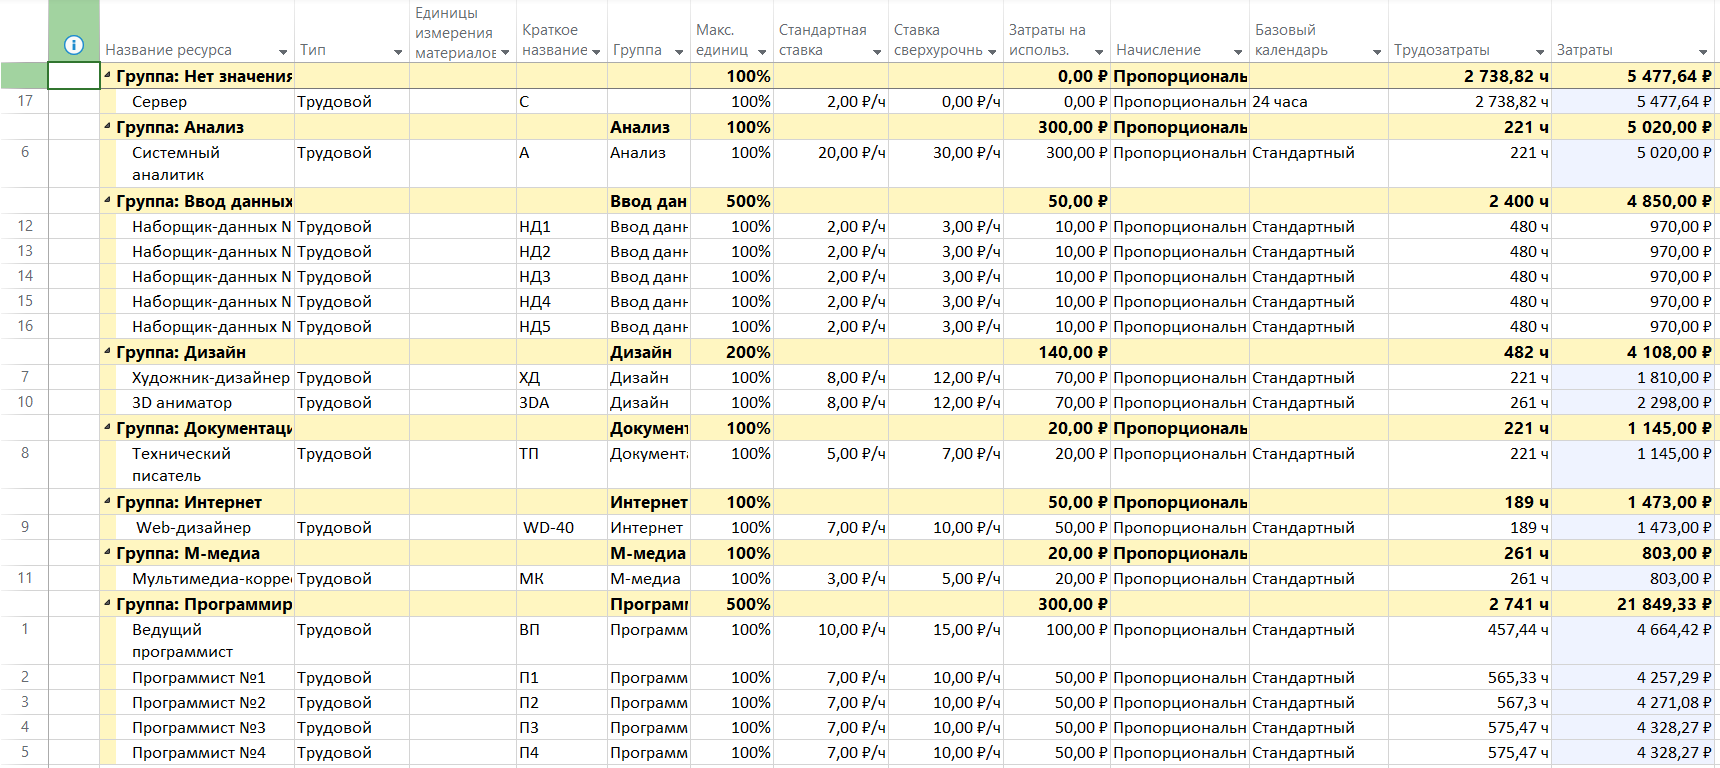
\includegraphics[width=\linewidth]{images/final_ochka_1.png}
	\caption{Сгруппированные ресурсы после применения мер оптимизации}
	\label{fig:7}
\end{figure}

В результате дата окончания проекта~---~22.07 и затраты на проект составили 47726 рублей, что укладывается в требования к проекту.

\section*{Выводы}

В результате принятых мер опитмизации проект укладывается в поставленных сроки (дата окончания 22.07) и финансы (затраты 47726 рублей). 

На рисунках~\ref{fig:8} и~\ref{fig:9} представлены круговые диаграммы трудозатрат и затрат соответственно.

\begin{figure}[H]
	\centering
	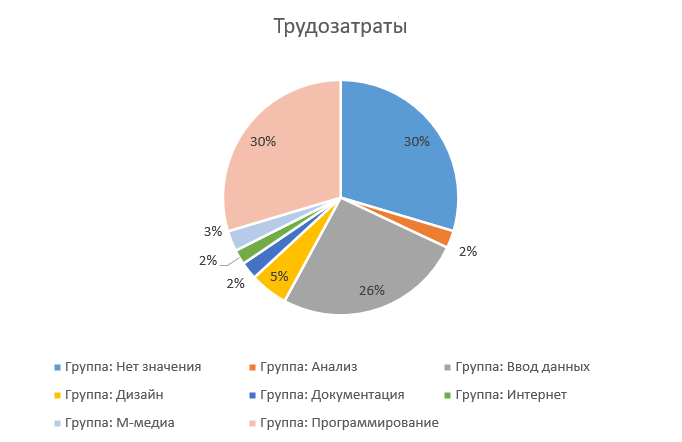
\includegraphics[width=\linewidth]{images/plot1.png}
	\caption{Круговая диаграмма трудозатрат проекта после оптимизации}
	\label{fig:8}
\end{figure}

\begin{figure}[H]
	\centering
	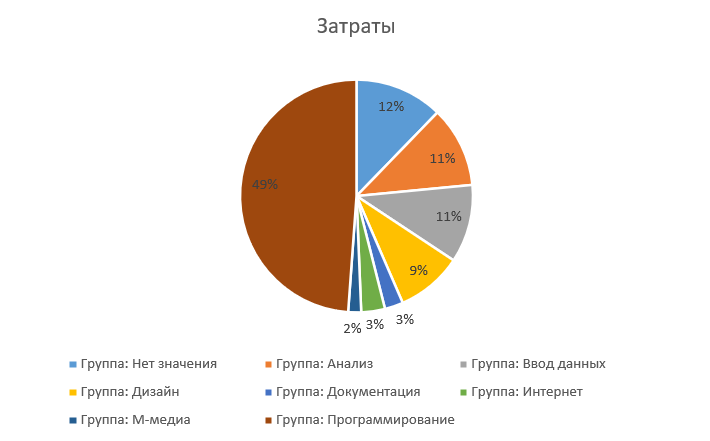
\includegraphics[width=\linewidth]{images/plot2.png}
	\caption{Круговая диаграмма затрат проекта после оптимизации}
	\label{fig:9}
\end{figure}

В результате применения оптимизационных мер, были достигнуты следующие изменения:
\begin{itemize}
	\item затраты на группу ресурсов "Программирование" уменьшились на 1\% от общей величины затрат и составляет теперь 49\%;
	\item затраты на использование сервера также сократились на один процент от общей величины затрат и составляет теперь 12\%;
	\item затраты на группы ресурсов "Анализ" и "Документация" увеличились на 1\% от общей величины затрат и составляют теперь 11\% и 3\% соответственно;
	\item трудозатраты групп "Программирование" и "Мультимедиа" увеличились на 1\% и составляют теперь 30\% и 3\% соответственно;
	\item время работы сервера уменьшилось на 2\% от общих трудозатрат и составляет теперь 30\%.
\end{itemize}